\documentclass{article}
\usepackage[utf8]{inputenc}
\usepackage{mathtools, amssymb}
\usepackage{float}
\usepackage{parskip}
\usepackage{wrapfig}
\usepackage{subcaption}
\usepackage{stmaryrd}


\usepackage[dvipsnames]{xcolor}
\title{Complex Analysis}
\author{dzackgarza }
\date{June 2017}
 
% Set this =0 to hide, =1 to show
\def\showanswers{1}
 
\newcommand{\hide}[1]{
   \ifnum\showanswers=1
 
   #1 \vspace{\baselineskip}
   \fi
 
   \ifnum\showanswers=0
   \vspace{2\baselineskip} \hspace{2cm}
   \fi
}

\begin{document}

\section{Notes}

\subsection{Definitions}

In these notes, $C$ generally denotes some closed contour, $\mathbb{H}$ is the upper half-plane, $C_R$ is a semicircle of radius $R$ in $\mathbb{H}$, $f$ will denote a complex function.


\begin{enumerate}
   \item \textbf{Analytic}
   
   $f$ is analytic at $z_0$ if it can be expanded as a convergent power series in some neighborhood of $z_0$.
   
   \item \textbf{Holomorphic}
   
   A function $f$ is holomorphic at a point $z_0$ if $f'(z_0)$ exists in a neighborhood of $z_0$.
   
   (Note - this is more than just being differentiable at a single point!)
   
   \textit{Big Theorem}: $f$ is a holomorphic complex function iff $f$ is analytic.
   
   \item \textbf{Meromorphic}
   
   Holomorphic, except for possibly a finite number of singularities.
   
   \item \textbf{Conformal}
   
   $f$ is conformal at $z_0$ if $f$ is analytic at $z_0$ and $f'(z_0) \neq 0$.
   
   \item \textbf{Harmonic}
   
   A function $u(x,y)$ is harmonic if it satisfies Laplace's equation, \[\Delta u = u_{xx} + u_{yy} = 0\]
\end{enumerate}

\subsection{What is the Complex Derivative?}

In small neighborhoods, the derivative of a function at a point rotates it by an angle $\Delta\theta$ and scales it by a real number $\lambda$  according to
\[\Delta\theta = \arg f'(z_0), ~\lambda = |f'(z_0)|\]

% Roots
\subsection{$n$th roots of a complex number}
The $n$th roots of $z_0$ are given by writing $z_0 = re^{i\theta}$, and are 
\[\zeta = \left\{ \sqrt[n]{r} \exp\left[{i\left( \frac{\theta}{n} + \frac{2k\pi}{n}\right)}\right] \mid k = 0,1,2,\cdots, n-1\right\}\]

or equivalently

\[\zeta = \left\{ \sqrt[n]{r}\omega_n^k \mid k = 0,1,2,\cdots, n-1\right\}~\text{where}~\omega_n = e^{\frac{2\pi i}{n}}\]

This can be derived by looking at $\left( re^{i\theta + 2k\pi}\right)^{\frac{1}{n}}$.

It is also useful to immediately recognize that $z^2+a = (z-i\sqrt{a})(z+i\sqrt{a})$.

% Cauchy-Riemann
\subsection{The Cauchy-Riemann Equations}

If $f(x+iy) = u(x,y) + iv(x,y)$ or $f(re^{i\theta}) = u(r,\theta) + iv(r,\theta)$, then $f$ is complex differentiable if $u,v$ satisfy 
\begin{align*}
    u_x &= v_y &\quad u_y &= -v_x \\
    ru_r &= v_\theta &\quad u_\theta &= -rv_r
\end{align*}

In this case, 
\[
f'(x+iy) = u_x(x,y) + iv_x(x,y)
\] 
or in polar coordinates, 
\[
f'(re^{i\theta}) = e^{i\theta}(u_r(r,\theta) + iv_r(r,\theta))
\]

\subsection{The Residue Theorem}


% Normal Residue
If $f$ is meromorphic inside of a closed contour $C$, then
\[ 
\oint_C f(z) dz = 2\pi i \sum_{z_k} \underset{z=z_k}{\text{Res}} f(z)
\]

where $\underset{z=z_k}{\text{Res}} f(z)$ is the coefficient of $z^{-1}$ in the Laurent expansion of $f$.

If $f$ is analytic everywhere in the interior of $C$, then $\oint_C f(z) dz = 0$.


% Residue at Infinity
If $f$ is meromorphic inside of a contour $C$ and analytic everywhere else, one can equivalently calculate the residue at infinity

\[ 
\oint_C f(z) dz = 2\pi i \sum_{z_k} \underset{z=0}{\text{Res}} ~z^{-2}f(z^{-1})
\]


% Computing Residues
\subsection{Computing Residues}

\subsubsection{Simple Poles}
If $z_0$ is a pole of order $m$, define $g(z) := (z-z_0)^m f(z)$.  

\textcolor{Blue}{If $g(z)$ is analytic and $g(z_0) \neq 0$}, then
\[
\underset{z=z_0}{\text{Res}} f(z) = \frac{\phi^{(m-1)}(z_0)}{(m-1)!}
\]

In the case where $m=1$, this reduces to
\[
\underset{z=z_0}{\text{Res}} f(z) = \phi(z_0)
\]

To compute residues this way, attempt to write $f$ in the form 

\[ f(z) = \frac{\phi(z)}{(z-z_0)^m}\]

where $\phi$ only needs to be analytic at $z_0$.

\subsubsection{Rational Functions}

If $f(z) = \frac{p(z)}{q(z)}$ where
\begin{enumerate}
   \item $p(z_0) \neq 0$
   \item $q(z_0) = 0$
   \item $q'(z_0) \neq 0$
\end{enumerate}

then the residue can be computed as

\[
\underset{z=z_0}{\text{Res}} \frac{p(z)}{q(z)} = \frac{p(z_0)}{q'(z_0)}
\]

\subsection{Computing Integrals}

When computing real integrals, the following contours can be useful:
% Insert contour pictures

One often needs bounds, which can come from the following lemmas

\textbf{The Arc Length Bound}
If $|f(z)| \leq M$ everywhere on $C$, then \[|\oint_C f(z) dz | \leq M L_C\] where $L_C$ is the length of $C$.

\textbf{Jordan's Lemma:}
If $f$ is analytic outside of a semicircle $C_R$ and $|f(z)| \leq M_R$ on $C_R$ where $M_R \rightarrow 0$, then 
\[ \int_{C_R} f(z) e^{iaz} dz \rightarrow 0\].

Can also be used for integrals of the form $\int f(z) \cos az dz$ or $\int f(z) \sin az dz$, just take real/imaginary parts of $e^{iaz}$ respectively.


\subsection{Conformal Maps}

\begin{enumerate}

    \item Linear Fractional Transformations:
        
    \[
    f(z) = \frac{az+b}{cz+d}\qquad f^{-1}(z) = \frac{-dz+b}{cz-a}
    \]
    
    
    \item $[z_1, z_2, z_3] \mapsto [w_1, w_2, w_3]$
    
    Every LFT is determined by its action on three points. Given 3 pairs points $z_i \mapsto w_i$, construct an LFT using the implicit equation
    \[
    \frac{(w-w_1)(w_2-w_3)}{(w-w_3)(w_2-w_1)} = \frac{(z-z_1)(z_2-z_3)}{(z-z_3)(z_2-z_1)}
    \]
    
    
   \item $z^k: \text{Wedge} \mapsto \mathbb{H}$
   
   Just multiplies the angle by $k$. If a wedge makes angle $\theta$, use $z^\frac{\pi}{\theta}$.
   
   It is useful to know that $z\mapsto z^2$ is equivalent to $(x,y) \mapsto (x^2-y^2, 2xy)$.
   
   \item $e^z: \mathbb{C} \mapsto \mathbb{C}$
   
\begin{tabular}{ l c l}
    Horizontal lines & $\mapsto$ & 
    rays from origin  \\
    Vertical lines &$\mapsto$ & 
    circles at origin  \\
    Rectangles &$\mapsto$ & 
    portions of wedges/sectors  \\
\end{tabular}
   
    \begin{figure}[H]
    \begin{subfigure}{\linewidth}
        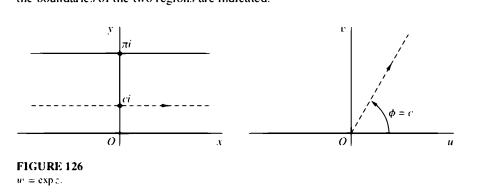
\includegraphics[width=\linewidth]{ez-line}\hfill
      \end{subfigure}\par\medskip
      \begin{subfigure}{\linewidth}
        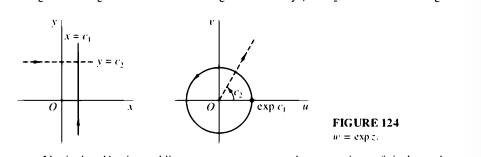
\includegraphics[width=\linewidth]{ez-grid}\hfill
      \end{subfigure}\par\medskip
      \begin{subfigure}{\linewidth}
        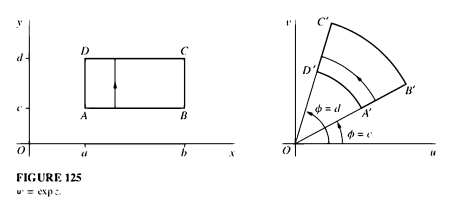
\includegraphics[width=\linewidth]{ez-rect}
      \end{subfigure}
    \end{figure}
    
    \item $\log: \mathbb{H} \mapsto \mathbb{R} + i[0, \pi]$
    
    Just the inverse of what the exponential map does.
    \begin{tabular}{ l c l}
        Rays & $\mapsto$ & 
        Horizontal Lines  \\
        Wedges &$\mapsto$ & 
        Horizontal Strips  \\
    \end{tabular}
    \begin{figure}[H]
        \centering
        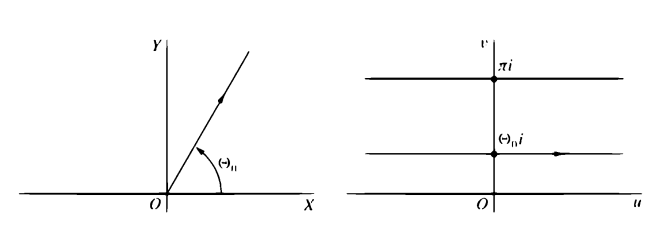
\includegraphics[width=\linewidth]{log}
        \caption{$z \mapsto \log z$}
    \end{figure}
    
    \item $\sin: [0, \pi/2] + i\mathbb{R} \mapsto \mathbb{H}_{\mathcal{R}(z)>0}$
    
    Maps the infinite strip to the first quadrant.
    
    \begin{figure}[H]
        \centering
        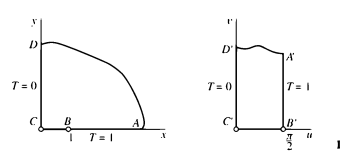
\includegraphics[width=\linewidth]{sin}
        \caption{$z \mapsfrom \sin w$}
    \end{figure}
    
    \item $z\mapsto\frac{i-z}{i+z}: \mathbb{H} \mapsto D^\circ$.
    
    \begin{tabular}{ l c l}
        $\mathbb{R}_{>0}$ & $\mapsto$ & 
        Upper half of $D^\circ$  \\
        $\mathbb{R}_{<0}$ &$\mapsto$ & 
        Bottom half of $D^\circ$  \\
    \end{tabular}
    
    Has inverse $w \mapsto i\frac{1-w}{1+w}$
    
    \item $z\mapsto z + z^{-1}: \partial D \mapsto \mathbb{R}$
    
    \begin{figure}[H]
        \centering
        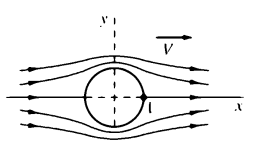
\includegraphics[width=0.5\linewidth]{fluid-cylinder}
        \caption{$z \mapsto z+z^{-1}$}
    \end{figure}
    
    Maps the boundary of the circle to the real axis, and the plane to $\mathbb{H}$.
    
    

   
\end{enumerate}

\subsection{Applications}

It is mostly important to know that composing a harmonic function on one domain with an analytic function produces a new harmonic function on the new domain.

Similarly, composing the solution to a boundary value problem on a domain with a conformal map produces a new solution to a new boundary problem in the new domain, where the new boundary is given by the conformal image of the old one.

The general technique is use solutions to the BVP on a simple domain $D$, and compose one or several conformal maps to map a given problem into $D$, then pull back the solution.

\subsubsection{Heat Flow: Steady Temperatures}

Generally interested in finding a harmonic function $T(x,y)$ which represents the steady-state temperature at any point. Usually given as a Dirichlet problem on a domain $D$ of the form

\begin{wrapfigure}{R}{0.35\textwidth}
\centering
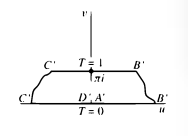
\includegraphics[width=0.35\textwidth]{heat-eqn.png}
\caption{$T(u,v) = \frac{1}{\pi}v$}
\end{wrapfigure}

\begin{align*}
    \Delta T &= 0 \\
    T(\partial D) &= f(\partial D)
\end{align*}

where $f$ is a given function that prescribes values on $\partial D$, the boundary of $D$.

Embed this in an analytic function with its harmonic conjugate to yield solutions of the form $F(x+iy) = T(x,y) + iS(x,y)$.



The \textbf{isotherms} are given by $T(x,y) = c$.

The \textbf{lines of flow} are given by $S(x,y) = c$.

\begin{wrapfigure}{R}{0.35\textwidth}
\centering
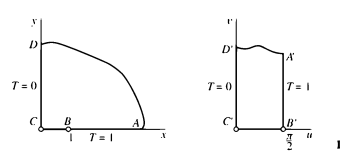
\includegraphics[width=0.35\textwidth]{sin.png}
\caption{$T(u,v) = \frac{2}{\pi}u$}
\end{wrapfigure}

Any easy solution on the domain $\mathbb{R} \times i[0,\pi]$ in the $u,v$ plane, where 

\begin{align*}
    T(x, 0) &= 0 \\
    T(x, \pi) &= 1
\end{align*} is given by $T(u,v) = \frac{1}{\pi}v$.

It is harmonic, as the imaginary part of the analytic $F(u+iv) = \frac{1}{\pi}(u+iv)$, since every analytic function has harmonic component functions.

Similar methods work with different domains, just pick a smooth interpolation between the boundary conditions.



\subsubsection{Fluid Flow}


\begin{wrapfigure}{R}{0.35\textwidth}
\centering
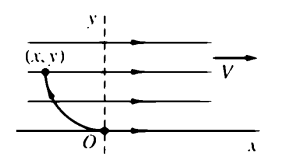
\includegraphics[width=0.35\textwidth]{fluid.png}
\caption{$T(u,v) = \frac{2}{\pi}u$}
\end{wrapfigure}
Write $F(z) = \phi(x,y) + i\psi(x,y)$. Then $F$ is the complex potential of the flow, $\overline{F'}$ is the velocity, and setting $\psi(x,y) = c$ yields the streamlines.

A solution in $\mathbb{H}$ is $F(z) = Az$ some some velocity $A$. Apply conformal mapping appropriately.



\begin{wrapfigure}{R}{0.35\textwidth}
\centering
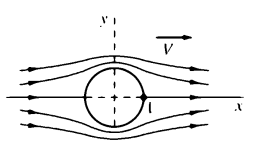
\includegraphics[width=0.35\textwidth]{fluid-cylinder.png}
\caption{$T(u,v) = \frac{2}{\pi}u$}
\end{wrapfigure}

\newpage
\subsection{Theorems}

\subsubsection{General Theorems}
\begin{enumerate}
   \item \textbf{Liouville's Theorem}: 
   
   If $f$ is entire and bounded on $\mathbb{C}$, then $f$ is constant.
   
   \item If $f$ is continuous in a region $D$, $f$ is bounded in $D$.
   
   \item If $f$ is differentiable at $z_0$, $f$ is continuous at $z_0$.
   
   Note - the converse need not hold!
   
   \item If $f = u + iv$ , where $u,v$ satisfy the Cauchy-Riemann equations \textbf{and} have continuous partials, then $f$ is differentiable.
   
   Note - continuous partials are not enough, consider $f(z) = |z|^2$.
   
   \item Rouche's Theorem
   
   If $p(z) = f(z) + g(z)$ and $|g(z)| < |f(z)|$ everywhere on $C$, then $f$ and $p$ have the same number of zeros with $C$.
   
   
   \item \textbf{The Argument Principle}
   
   If $f$ is analytic on a closed contour $C$ and meromorphic within $C$, then
   \[
   W := \frac{1}{2\pi}\Delta_C \arg f(z) = Z - P
   \]
   
   \textit{Proof:} Evaluate the integral $\oint_C \frac{f'(z)}{f(z)} dz$ first by parameterizing, changing to polar, and using the FTC, and second by using residues directly from the Laurent series.
   
   \item \textbf{The Main Story}: The following are equivalent
   
   \begin{itemize}
       \item $f$ is continuous
       \item $f'$ exists
       \item $f$ is analytic
       \item $f$ is conformal
       \item $f$ satisfies the Cauchy-Riemann equations
   \end{itemize}
   
\end{enumerate}

\subsubsection{Theorems About Analytic Functions}
\begin{enumerate}

    \item If $f$ is analytic on $D$, then $\oint_C f(z) dz = 0$ for any closed contour $C \subset D$.
    
    Note: this does not require $f$ to be $f'$ to be continuous on $C$.
  
   \item \textbf{Maximum Modulus Principle}
   
   If $f$ is analytic in a region $D$ and not constant, then $|f(z)|$ attains its maximum on $\partial D$.
   
   \item If $f$ is analytic, then $f^{(n)}$ is analytic for every $n$. If $f = u(x,y) + iv(x,y)$, then all partials of $u,v$ are continuous.
   
   \item If $f$ is analytic at $z_0$ and $f'(z_0) \neq 0$, then $f$ is conformal at $z_0$.
   
   \item If $f = u+iv$ is analytic, then $u,v$ are harmonic conjugates.
   
   \item If $f$ is holomorphic, $f$ is $C_\infty$ (smooth).
   
   \item If $f$ is analytic, $f$ is holomorphic.
   
   \textit{Proof:} Since $f$ has a power series expansion at $z_0$, its derivative is given by the term-by-term differentiation of this series.
   
\end{enumerate}


\subsection{Some Useful Formulae}

\[
f_{x_0}(x) = f(x_0) + f'(x_0)(x-x_0) + \frac{1}{2!}f''(x_0)(x-x_0)^2 + \cdots
\]

\[ 
\frac{1}{1-z} = \sum_k z^k
\]

\[ 
e^z = \sum_k \frac{1}{k!} z^k 
\]

\[
\left(\sum_i a_i z^i \right) \left( \sum_j b_j z^j\right) = \sum_n \left( \sum\limits_{i+j=n}a_ib_j \right) z^n
\]
\begin{align*}
%   
\cos z 
&= \frac{1}{2}(e^{iz} + e^{-iz})
&
&= 1 - \frac{z^2}{2!} + \frac{z^4}{4!} - \cdots \\
%
\cosh z 
&= \frac{1}{2}(e^{z} + e^{-z}) 
&= \cos iz 
&= 1 + \frac{z^2}{2!} + \frac{z^4}{4!} + \cdots \\
%
\sin z 
&= \frac{1}{2i}(e^{iz} - e^{-iz}) 
&
&= z - \frac{z^3}{3!} + \frac{z^4}{4!} - \cdots \\
%
\sinh z 
&= \frac{1}{2}(e^{z} - e^{-z}) 
&= -i\sin iz 
&= z + \frac{z^3}{3!} + \frac{z^4}{4!} + \cdots \\
\end{align*}
Mnemonic: just remember that cosine is an even function, and that the even terms of $e^z$ are kept. Similarly, sine is an odd function, so keep the odd terms of $e^z$.

\textbf{Harmonic Conjugate}
\[ v(x,y) = \int_{(0,0)}^{(x,y)} -u_t(s,t)ds + u_s(s,t)dt\]

\textbf{The Gamma Function}
\[ \Gamma(z) = \int_0^\infty x^{z-1} e^{-x} dx \]

Useful to know: $\Gamma(\frac{1}{2}) = \sqrt\pi$.


%%% Questions
\section{Question}
\begin{enumerate}
   \item True or False: If $f$ is analytic and bounded in $\mathbb{H}$, then $f$ is constant on $\mathbb{H}$.
   \hide{
   False: Take $f(z) = e^{-z}$, where $|f(z)| \leq 1$ in $\mathbb{H}$.
   }
 
   \item Compute $\int_{-\infty}^{\infty} \frac{\sin x}{x(x^2+a^2)}dx$
   \hide{
   Two semicircles needed to avoid singularity at zero. Limit equals the residue at zero, solution is $\pi (\frac{1}{a^2} - \frac{e^{-a}}{a^2})$.
   }
   
   \item Compute $\int_0^{2\pi} \frac{1}{2+\cos\theta}d\theta$
   \hide{
   Cosine sub, solution is $\frac{2\pi}{\sqrt{3}}$
   }
   
   \item Find the first three terms of the Laurent expansion of $\frac{e^z+1}{e^z-1}$.
   \hide{
   Equals $2z^{-1} + 0 + 6^{-1}z + \cdots$
   }
   
  \item Compute $\int_{S_1} \frac{1}{z^2+z-1}dz$
   \hide{
    Equals $i\frac{2\pi}{5}$
   }
   
  \item True or false: If f is analytic on the unit disk $E = \{z : |z| < 1\}$, then there exists an $a \in E$ such
  that $|f (a)| \geq |f (0)|$.
   \hide{
   True, by the maximum modulus principal. Suppose otherwise. Then $f(0)$ is a maximum of $f$ inside $S_1$. But by the MMP, $f$ must attain its maximum on $\partial S_1$.
   }
   
   \item Prove that if $f(z)$ and $f (\bar{z})$ are both analytic on a domain D, then f is constant on D
   \hide{
   Analytic $\implies$ Cauchy-Riemann equations are satisfied. Also have the identity $f' = u_x + iv_x$, and $f' = 0$ $\implies$ $f$ is constant.
   }
   
\end{enumerate}
\end{document}
